%%%%%%%%%%%%%%%%%%%%%%%%%%%%%%%%%%%%%%%%%%%%%%%%%%%%%%%%%%%%%%%%%%%%%%%%%%%%%%%%%%%%%%%%%%%%%%%%%
%
% Document:     Data Management  product tree
%
%%%%%%%%%%%%%%%%%%%%%%%%%%%%%%%%%%%%%%%%%%%%%%%%%%%%%%%%%%%%%%%%%%%%%%%%%%%%%%
\documentclass{article}
\usepackage{times,layouts}
\usepackage{tikz,hyperref,amsmath}
\usetikzlibrary{positioning,arrows,shapes,decorations.shapes,shapes.arrows}
\usetikzlibrary{backgrounds,calc}
\usepackage[paperwidth=1441.9999999999998pt,paperheight=516pt,
left=-2mm,top=3mm,bottom=0mm,right=0mm,
noheadfoot,marginparwidth=0pt,includemp=false,
textwidth=30cm,textheight=50mm]{geometry}
\newcommand\showpage{%
\setlayoutscale{0.5}\setlabelfont{\tiny}\printheadingsfalse\printparametersfalse
\currentpage\pagedesign}
\hypersetup{pdftitle={Data Management products }, pdfsubject={Diagram illustrating the
                products in LSST Data Management }, pdfauthor={Extracted from MagicDraw}}
\tikzstyle{tbox}=[rectangle,text centered, text width=30mm]
\tikzstyle{wbbox}=[rectangle, rounded corners=3pt, draw=black, top color=blue!50!white,
                    bottom color=white, very thick, minimum height=40pt, inner sep=2pt,
                    text centered, text width=30mm]
\tikzstyle{pbox}=[rectangle, rounded corners=3pt, draw=black, top
 color=yellow!50!white, bottom color=white, very thick,
 minimum height=36pt, inner sep=3pt, text centered, text width=35mm]
\tikzstyle{pline}=[-, thick]
\begin{document}
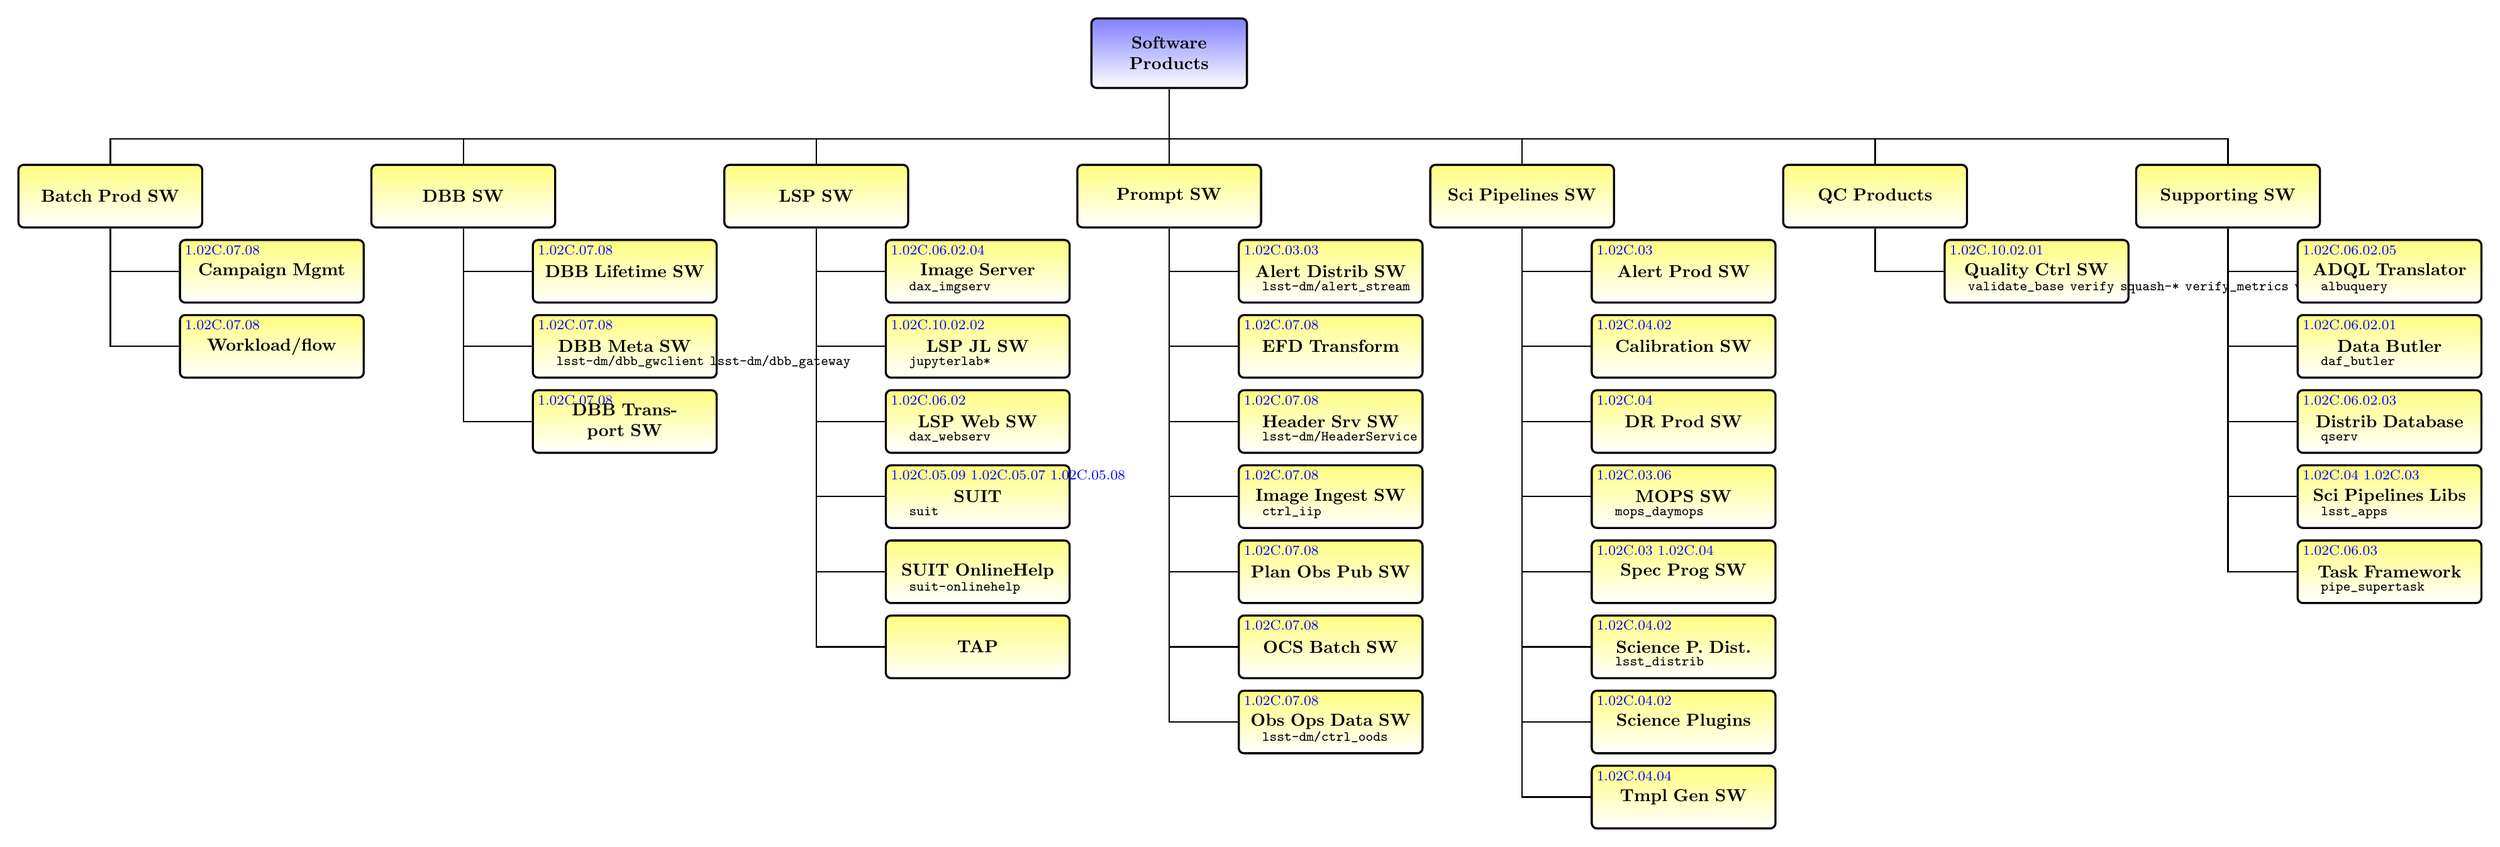
\begin{tikzpicture}[node distance=0mm]


\node (BPP) [pbox, 
] {\textbf{Batch Prod SW
} };\node [below right] at (BPP.north west) {\footnotesize \color{blue}} ;

\node (CMPGN) [pbox,below right=6pt and -14pt of BPP] {\textbf{Campaign Mgmt
} };\node [below right] at (CMPGN.north west) {\footnotesize \color{blue}1.02C.07.08} ;

 \draw[pline] (BPP.south) -| ++(0,0) |- (CMPGN.west); 
\node (WLWF) [pbox,below=6pt of CMPGN] {\textbf{Workload/flow
} };\node [below right] at (WLWF.north west) {\footnotesize \color{blue}1.02C.07.08} ;

 \draw[pline] (BPP.south) -| ++(0,0) |- (WLWF.west); 
\node (DBB) [pbox, 
right=96pt of BPP] {\textbf{DBB SW
} };\node [below right] at (DBB.north west) {\footnotesize \color{blue}} ;

\node (DBBLIFE) [pbox,below right=6pt and -14pt of DBB] {\textbf{DBB Lifetime SW
} };\node [below right] at (DBBLIFE.north west) {\footnotesize \color{blue}1.02C.07.08} ;

 \draw[pline] (DBB.south) -| ++(0,0) |- (DBBLIFE.west); 
\node (DBBMD) [pbox,below=6pt of DBBLIFE] {\textbf{DBB Meta SW
} };\node [below right] at (DBBMD.north west) {\footnotesize \color{blue}1.02C.07.08} ;
\node (DBBMDpkg) [tbox,below=3mm of DBBMD.north] {{\footnotesize \color{black} \begin{verbatim} lsst-dm/dbb_gwclient lsst-dm/dbb_gateway \end{verbatim} }  };

 \draw[pline] (DBB.south) -| ++(0,0) |- (DBBMD.west); 
\node (DBBTR) [pbox,below=6pt of DBBMD] {\textbf{DBB Transport SW
} };\node [below right] at (DBBTR.north west) {\footnotesize \color{blue}1.02C.07.08} ;

 \draw[pline] (DBB.south) -| ++(0,0) |- (DBBTR.west); 
\node (LSP) [pbox, 
right=96pt of DBB] {\textbf{LSP SW
} };\node [below right] at (LSP.north west) {\footnotesize \color{blue}} ;

\node (DAXIMG) [pbox,below right=6pt and -14pt of LSP] {\textbf{Image Server
} };\node [below right] at (DAXIMG.north west) {\footnotesize \color{blue}1.02C.06.02.04} ;
\node (DAXIMGpkg) [tbox,below=3mm of DAXIMG.north] {{\footnotesize \color{black} \begin{verbatim} dax_imgserv \end{verbatim} }  };

 \draw[pline] (LSP.south) -| ++(0,0) |- (DAXIMG.west); 
\node (LSPJL) [pbox,below=6pt of DAXIMG] {\textbf{LSP JL SW
} };\node [below right] at (LSPJL.north west) {\footnotesize \color{blue}1.02C.10.02.02} ;
\node (LSPJLpkg) [tbox,below=3mm of LSPJL.north] {{\footnotesize \color{black} \begin{verbatim} jupyterlab* \end{verbatim} }  };

 \draw[pline] (LSP.south) -| ++(0,0) |- (LSPJL.west); 
\node (LSPWEB) [pbox,below=6pt of LSPJL] {\textbf{LSP Web SW
} };\node [below right] at (LSPWEB.north west) {\footnotesize \color{blue}1.02C.06.02} ;
\node (LSPWEBpkg) [tbox,below=3mm of LSPWEB.north] {{\footnotesize \color{black} \begin{verbatim} dax_webserv \end{verbatim} }  };

 \draw[pline] (LSP.south) -| ++(0,0) |- (LSPWEB.west); 
\node (SUIT) [pbox,below=6pt of LSPWEB] {\textbf{SUIT
} };\node [below right] at (SUIT.north west) {\footnotesize \color{blue}1.02C.05.09 1.02C.05.07 1.02C.05.08} ;
\node (SUITpkg) [tbox,below=3mm of SUIT.north] {{\footnotesize \color{black} \begin{verbatim} suit \end{verbatim} }  };

 \draw[pline] (LSP.south) -| ++(0,0) |- (SUIT.west); 
\node (SUITOH) [pbox,below=6pt of SUIT] {\textbf{SUIT OnlineHelp
} };\node [below right] at (SUITOH.north west) {\footnotesize \color{blue}} ;
\node (SUITOHpkg) [tbox,below=3mm of SUITOH.north] {{\footnotesize \color{black} \begin{verbatim} suit-onlinehelp \end{verbatim} }  };

 \draw[pline] (LSP.south) -| ++(0,0) |- (SUITOH.west); 
\node (TAPSW) [pbox,below=6pt of SUITOH] {\textbf{TAP
} };\node [below right] at (TAPSW.north west) {\footnotesize \color{blue}} ;

 \draw[pline] (LSP.south) -| ++(0,0) |- (TAPSW.west); 
\node (PR) [pbox, 
right=96pt of LSP] {\textbf{Prompt SW
} };\node [below right] at (PR.north west) {\footnotesize \color{blue}} ;

\node (ALRTDSTR) [pbox,below right=6pt and -14pt of PR] {\textbf{Alert Distrib SW
} };\node [below right] at (ALRTDSTR.north west) {\footnotesize \color{blue}1.02C.03.03} ;
\node (ALRTDSTRpkg) [tbox,below=3mm of ALRTDSTR.north] {{\footnotesize \color{black} \begin{verbatim} lsst-dm/alert_stream \end{verbatim} }  };

 \draw[pline] (PR.south) -| ++(0,0) |- (ALRTDSTR.west); 
\node (EFDT) [pbox,below=6pt of ALRTDSTR] {\textbf{EFD Transform
} };\node [below right] at (EFDT.north west) {\footnotesize \color{blue}1.02C.07.08} ;

 \draw[pline] (PR.south) -| ++(0,0) |- (EFDT.west); 
\node (HEADER) [pbox,below=6pt of EFDT] {\textbf{Header Srv SW
} };\node [below right] at (HEADER.north west) {\footnotesize \color{blue}1.02C.07.08} ;
\node (HEADERpkg) [tbox,below=3mm of HEADER.north] {{\footnotesize \color{black} \begin{verbatim} lsst-dm/HeaderService \end{verbatim} }  };

 \draw[pline] (PR.south) -| ++(0,0) |- (HEADER.west); 
\node (IIP) [pbox,below=6pt of HEADER] {\textbf{Image Ingest SW
} };\node [below right] at (IIP.north west) {\footnotesize \color{blue}1.02C.07.08} ;
\node (IIPpkg) [tbox,below=3mm of IIP.north] {{\footnotesize \color{black} \begin{verbatim} ctrl_iip \end{verbatim} }  };

 \draw[pline] (PR.south) -| ++(0,0) |- (IIP.west); 
\node (OBSPUB) [pbox,below=6pt of IIP] {\textbf{Plan Obs Pub SW
} };\node [below right] at (OBSPUB.north west) {\footnotesize \color{blue}1.02C.07.08} ;

 \draw[pline] (PR.south) -| ++(0,0) |- (OBSPUB.west); 
\node (OCSBAT) [pbox,below=6pt of OBSPUB] {\textbf{OCS Batch SW
} };\node [below right] at (OCSBAT.north west) {\footnotesize \color{blue}1.02C.07.08} ;

 \draw[pline] (PR.south) -| ++(0,0) |- (OCSBAT.west); 
\node (OODS) [pbox,below=6pt of OCSBAT] {\textbf{Obs Ops Data SW
} };\node [below right] at (OODS.north west) {\footnotesize \color{blue}1.02C.07.08} ;
\node (OODSpkg) [tbox,below=3mm of OODS.north] {{\footnotesize \color{black} \begin{verbatim} lsst-dm/ctrl_oods \end{verbatim} }  };

 \draw[pline] (PR.south) -| ++(0,0) |- (OODS.west); 
\node (PRODN) [pbox, 
right=96pt of PR] {\textbf{Sci Pipelines SW
} };\node [below right] at (PRODN.north west) {\footnotesize \color{blue}} ;

\node (APPRMPT) [pbox,below right=6pt and -14pt of PRODN] {\textbf{Alert Prod SW
} };\node [below right] at (APPRMPT.north west) {\footnotesize \color{blue}1.02C.03} ;

 \draw[pline] (PRODN.south) -| ++(0,0) |- (APPRMPT.west); 
\node (DMCAL) [pbox,below=6pt of APPRMPT] {\textbf{Calibration SW
} };\node [below right] at (DMCAL.north west) {\footnotesize \color{blue}1.02C.04.02} ;

 \draw[pline] (PRODN.south) -| ++(0,0) |- (DMCAL.west); 
\node (DRP) [pbox,below=6pt of DMCAL] {\textbf{DR Prod SW
} };\node [below right] at (DRP.north west) {\footnotesize \color{blue}1.02C.04} ;

 \draw[pline] (PRODN.south) -| ++(0,0) |- (DRP.west); 
\node (MOPS) [pbox,below=6pt of DRP] {\textbf{MOPS SW
} };\node [below right] at (MOPS.north west) {\footnotesize \color{blue}1.02C.03.06} ;
\node (MOPSpkg) [tbox,below=3mm of MOPS.north] {{\footnotesize \color{black} \begin{verbatim} mops_daymops \end{verbatim} }  };

 \draw[pline] (PRODN.south) -| ++(0,0) |- (MOPS.west); 
\node (SP) [pbox,below=6pt of MOPS] {\textbf{Spec Prog SW
} };\node [below right] at (SP.north west) {\footnotesize \color{blue}1.02C.03 1.02C.04} ;

 \draw[pline] (PRODN.south) -| ++(0,0) |- (SP.west); 
\node (SPDIST) [pbox,below=6pt of SP] {\textbf{Science P. Dist.
} };\node [below right] at (SPDIST.north west) {\footnotesize \color{blue}1.02C.04.02} ;
\node (SPDISTpkg) [tbox,below=3mm of SPDIST.north] {{\footnotesize \color{black} \begin{verbatim} lsst_distrib \end{verbatim} }  };

 \draw[pline] (PRODN.south) -| ++(0,0) |- (SPDIST.west); 
\node (SPLUG) [pbox,below=6pt of SPDIST] {\textbf{Science Plugins
} };\node [below right] at (SPLUG.north west) {\footnotesize \color{blue}1.02C.04.02} ;

 \draw[pline] (PRODN.south) -| ++(0,0) |- (SPLUG.west); 
\node (TMPLGEN) [pbox,below=6pt of SPLUG] {\textbf{Tmpl Gen SW
} };\node [below right] at (TMPLGEN.north west) {\footnotesize \color{blue}1.02C.04.04} ;

 \draw[pline] (PRODN.south) -| ++(0,0) |- (TMPLGEN.west); 
\node (QC) [pbox, 
right=96pt of PRODN] {\textbf{QC Products
} };\node [below right] at (QC.north west) {\footnotesize \color{blue}} ;

\node (QCSW) [pbox,below right=6pt and -14pt of QC] {\textbf{Quality Ctrl SW
} };\node [below right] at (QCSW.north west) {\footnotesize \color{blue}1.02C.10.02.01} ;
\node (QCSWpkg) [tbox,below=3mm of QCSW.north] {{\footnotesize \color{black} \begin{verbatim} validate_base verify squash-* verify_metrics validate_drp \end{verbatim} }  };

 \draw[pline] (QC.south) -| ++(0,0) |- (QCSW.west); 
\node (SUPPSW) [pbox, 
right=96pt of QC] {\textbf{Supporting SW
} };\node [below right] at (SUPPSW.north west) {\footnotesize \color{blue}} ;

\node (ADQL) [pbox,below right=6pt and -14pt of SUPPSW] {\textbf{ADQL Translator
} };\node [below right] at (ADQL.north west) {\footnotesize \color{blue}1.02C.06.02.05} ;
\node (ADQLpkg) [tbox,below=3mm of ADQL.north] {{\footnotesize \color{black} \begin{verbatim} albuquery \end{verbatim} }  };

 \draw[pline] (SUPPSW.south) -| ++(0,0) |- (ADQL.west); 
\node (BUTLER) [pbox,below=6pt of ADQL] {\textbf{Data Butler
} };\node [below right] at (BUTLER.north west) {\footnotesize \color{blue}1.02C.06.02.01} ;
\node (BUTLERpkg) [tbox,below=3mm of BUTLER.north] {{\footnotesize \color{black} \begin{verbatim} daf_butler \end{verbatim} }  };

 \draw[pline] (SUPPSW.south) -| ++(0,0) |- (BUTLER.west); 
\node (QSERV) [pbox,below=6pt of BUTLER] {\textbf{Distrib Database
} };\node [below right] at (QSERV.north west) {\footnotesize \color{blue}1.02C.06.02.03} ;
\node (QSERVpkg) [tbox,below=3mm of QSERV.north] {{\footnotesize \color{black} \begin{verbatim} qserv \end{verbatim} }  };

 \draw[pline] (SUPPSW.south) -| ++(0,0) |- (QSERV.west); 
\node (SCIPIPE) [pbox,below=6pt of QSERV] {\textbf{Sci Pipelines Libs
} };\node [below right] at (SCIPIPE.north west) {\footnotesize \color{blue}1.02C.04 1.02C.03} ;
\node (SCIPIPEpkg) [tbox,below=3mm of SCIPIPE.north] {{\footnotesize \color{black} \begin{verbatim} lsst_apps \end{verbatim} }  };

 \draw[pline] (SUPPSW.south) -| ++(0,0) |- (SCIPIPE.west); 
\node (TXF) [pbox,below=6pt of SCIPIPE] {\textbf{Task Framework
} };\node [below right] at (TXF.north west) {\footnotesize \color{blue}1.02C.06.03} ;
\node (TXFpkg) [tbox,below=3mm of TXF.north] {{\footnotesize \color{black} \begin{verbatim} pipe_supertask \end{verbatim} }  };

 \draw[pline] (SUPPSW.south) -| ++(0,0) |- (TXF.west); 
\node (DMSW) [wbbox, above=43pt of PR]{\textbf{Software Products}};
 \draw[pline]   (BPP.north) -- ++(0.0,0.5) -| (DMSW.south) ; 
 \draw[pline]   (DBB.north) -- ++(0.0,0.5) -| (DMSW.south) ; 
 \draw[pline]   (LSP.north) -- ++(0.0,0.5) -| (DMSW.south) ; 
 \draw[pline]   (PR.north) -- ++(0.0,0.5) -| (DMSW.south) ; 
 \draw[pline]   (PRODN.north) -- ++(0.0,0.5) -| (DMSW.south) ; 
 \draw[pline]   (QC.north) -- ++(0.0,0.5) -| (DMSW.south) ; 
 \draw[pline]   (SUPPSW.north) -- ++(0.0,0.5) -| (DMSW.south) ; 

\end{tikzpicture}
\end{document}
